\documentclass[stu,12pt,floatsintext]{apa7}
% Document class: student paper, 12pt, with figures/tables in text.

\usepackage[american]{babel}
\usepackage{csquotes} 
\usepackage[style=apa,sortcites=true,sorting=nyt,backend=biber]{biblatex}
\DeclareLanguageMapping{american}{american-apa}
\addbibresource{references.bib} % Ensure your bibliography file is named references.bib

\usepackage[T1]{fontenc} 
\usepackage{mathptmx}
\usepackage{amsmath}

% Title page information
\title{When Stories Sync Our Minds: EEG-fMRI Insights into Narrative vs. Non-Narrative Brain Dynamics}
\shorttitle{PSYC 42350 Final Project}
\author{Sam}
\duedate{March 12, 2025}
\course{PSYC 42350}
\affiliation{University of Chicago}
\professor{Dr. Wilma Bainbridge \& Dr. Monica Rosenberg}

\abstract{Narrative stimuli have been shown to evoke strongly synchronized brain responses, yet the extent to which they also align cross-modal neural representations remains less understood. To compare the shared neural synchrony and cross-modal alignment of neural signals between narrative and non-narrative stimuli, this study leveraged an open-access dataset featuring simultaneous EEG-fMRI recordings of participants viewing narrative (e.g., \emph{Despicable Me}) and non-narrative (\emph{Inscapes}) clips using two complementary analyses: 1) inter-subject correlation (ISC) of fMRI signals (to measure shared neural synchrony) and 2) cross-modal representational similarity analysis (RSA; to assess the alignment of EEG and fMRI patterns). The ISC results revealed that coherent narratives significantly enhanced synchrony in high-order cortical networks, including the Control/Frontoparietal and Default Mode networks, consistent with the notion that plot coherence and emotional structure drive inter-subject alignment. In contrast, RSA demonstrated only modest differences between narrative and non-narrative conditions, with no statistically significant cross-modal alignment. Additionally, classification based on RSA features yielded near-chance accuracy (52.8\%), indicating that the current parameters did not robustly discriminate between narrative and non-narrative stimuli. These findings suggest that while narrative content powerfully synchronizes brain activity across individuals, further methodological refinements may be needed to capture the finer-grained temporal-spatial dynamics that could more effectively reveal cross-modal representational similarities.}

\begin{document}
\maketitle

\section{Introduction}
Narratives have long served as a cornerstone of human communication, enabling the sharing of experiences, the transmission of knowledge, and the fostering of empathy (\cite{jaaskelainen_neural_2020}; \cite{nguyen_shared_2019}). Unlike isolated, controlled stimuli typically used in laboratory experiments, naturalistic narratives unfold over extended periods and engage multiple cognitive processes simultaneously. These processes include attention, memory, language comprehension, and emotion, all of which contribute to the creation of a rich, coherent experience (\cite{regev_propagation_2019}).

Many previous studies have shown remarkably synchronized patterns of activity when people are exposed to the same narrative, be it a film, a story, or a spoken discourse (e.g., \cite{nastase_measuring_2019}; \cite{yeshurun_same_2017}). For example, early work by \textcite{hasson_enhanced_2008} revealed that viewing a narrative film leads to inter-subject correlations (ISC) in brain regions that span from early sensory areas to high-order associative networks such as the Default Mode Network (DMN) and frontoparietal regions. These findings suggest that narratives not only drive consistent sensory processing, but also induce higher-order cognitive alignment among viewers.

Not all stimuli generate this kind of broad synchrony – narrative coherence appears to be key. Research contrasting narrative vs. non-narrative content suggests that only richly structured stories reliably engage higher-order cortical networks (e.g.,. \cite{dini_higher_2023}; \cite{naci_common_2014}). Contrasting non-narrative stimuli provides an essential control condition to determine whether high-level neural synchrony truly stems from narrative structure or merely from shared perceptual input, such as color, motion, or other low-level features. If non-narrative stimuli yield lower synchronization in high-order networks compared to coherent narratives, it supports the notion that plot coherence and the unfolding of a meaningful storyline are crucial for inducing inter-subject alignment.

More recent studies have extended these observations by incorporating simultaneous EEG-fMRI methodologies. This multimodal approach takes advantage of the high temporal resolution of EEG to capture rapid neural dynamics and the high spatial resolution of fMRI to localize these processes within specific brain networks (\cite{haufe_elucidating_2018}). Recent studies have demonstrated the value of such combined recordings. For example, simultaneous EEG fMRI recordings during movie viewing show that the two signals are meaningfully related, with certain fluctuations in the EEG frequency band correlated with BOLD activity in the corresponding brain regions (\cite{haufe_elucidating_2018}). These cross-modal correspondences suggest that a common underlying neural process (e.g. narrative event processing) can be detected in both electrical and hemodynamic measures. To formally link activity patterns between modalities and across subjects, researchers are increasingly using representational similarity analysis (RSA). RSA can quantify whether different data (e.g., EEG vs. fMRI, or brain responses vs. narrative content) share a similar information structure and allow researchers to bridge across different brain measures and even different sensory formats to isolate the common representational and neural dynamics that define narrative experiences.

Amid this background, this study aims to compare neural synchrony between narrative and non-narrative stimuli using an open-source neuroimaing data of naturalistic viewing using simultaneous EEG-fMRI. Specifically, it seeks to address the following two research questions: \textbf{1) Do narratives evoke stronger inter-subject correlation in fMRI? 2) Does cross-modal EEG–fMRI RSA differ between narrative vs. non-narrative? Additionally, can multimodal signals classify if a segment is narrative or not?} By employing ISC to quantify shared neural processing and RSA to examine the alignment of neural representations across modalities, this study aim to determine whether coherent narratives lead to enhanced neural synchrony and if such alignment can be robustly detected. This multimodal approach offers a unique opportunity to capture both the temporal and spatial dynamics associated with narrative comprehension, thereby advancing our understanding of the neural mechanisms that underlie shared human experiences.

\section{Method}
\subsection{Dataset}
The dataset used in this study (\cite{telesford_open-access_2023}) is an open-access resource for naturalistic viewing using simultaneous EEG-fMRI. The dataset comprises recordings from 22 healthy adults (age 23–51, with a mean age of approximately 36.8 years; roughly 50\% male). All participants had no history of psychiatric or neurological illnesses.

Data were acquired during two scanning sessions, with intervals between sessions ranging from 2 to 354 days (mean interval of 38.2 days). Each session included several recording settings. In addition to simultaneous EEG-fMRI recordings, separate EEG recordings were obtained in non-MRI environments (``Outside'' and ``Scanner OFF'') to evaluate the effects of the scanner environment on the EEG signal. 

The experimental paradigm encompassed a variety of tasks: a flickering checkerboard stimulus (presented at 12 Hz) to probe visual cortex responsiveness, a resting state condition where participants fixated on a white cross against a black background, and naturalistic viewing of video stimuli. Naturalistic stimuli included an extended version of the computer-generated animation \textit{Inscapes} (10 minutes), as well as multiple movie clips such as a 10-minute segment from \textit{Despicable Me} (presented in both English and Hungarian), a short film titled \textit{The Present}, and several 5-minute monkey videos selected from an established video database.

The fMRI data were preprocessed using the Connectome Computation System (CCS). Anatomical images underwent skull stripping, segmentation, and registration to the MNI152 template using tools such as the Brain Extraction Toolbox (BET) and Freesurfer. Functional data were processed by discarding the initial five volumes to allow magnetization stabilization, followed by despiking, slice timing correction, and motion correction. The functional images were then skull-stripped and aligned with the anatomical images using boundary-based registration. Nuisance variables, including cerebrospinal fluid (CSF), white matter (WM) signals, and motion parameters, were regressed out from the time series. Finally, the data were temporally filtered (0.01–0.1 Hz) and spatially smoothed using a 6 mm full-width half-maximum (FWHM) Gaussian kernel, with time series subsequently extracted from 400 regions of interest based on the Schaefer 400 atlas.

This comprehensive dataset provides a rich foundation for exploring the neural mechanisms underlying naturalistic narrative processing. In the present study, I specifically focus on two sets of naturalistic stimuli: abstract, computer-generated animation \textit{Inscapes} and segments from the film \textit{Despicable Me}. These two naturalistic stimuli enables the comparison of the neural synchrony and representational dynamics elicited by narrative versus non-narrative visual content.

\subsection{Data Analysis}
This study employs two complementary analytic techniques—inter-subject correlation (ISC) and representational similarity analysis (RSA)—to investigate neural synchrony and cross-modal representational alignment in a naturalistic EEG-fMRI dataset. The following sections describe the procedures implemented for each analysis, including data loading, segmentation, and subsequent statistical computations.

\subsubsection{ISC}
ISC measures the similarity of neural responses across individuals when exposed to the same naturalistic stimulus. In this part, only the fMRI time series were used to compute ISC. The preprocessed fMRI data were first loaded from the 4D NifTI file of each subject and flattened into a 2D matrix (time points $\times$ voxels). Data were acquired in MNI space with a resolution of 3\,mm. For each subject, the time course of each voxel was correlated with the mean time course of all other subjects to generate an individual ISC map. The resulting ISC maps were then aggregated within predefined regions corresponding to the 17 Yeo networks (e.g., visual, control, and default mode networks; \cite{thomas_yeo_organization_2011}). To determine statistical significance, permutation tests were conducted by circularly shifting time series to generate a null distribution. The resulting $p$-values were then corrected for multiple comparisons using false discovery rate (FDR) procedures.

\subsubsection{Cross-Modal RSA}
RSA provides a multivariate approach to compare the representational geometry of neural responses across different modalities. In this study, data from both EEG and fMRI, and from two conditions (narrative vs. non-narrative), were segmented into fixed-length windows of 10 seconds. For each segment, the average neural pattern was computed and then used to construct a representational dissimilarity matrix (RDM). In this process, the dissimilarity between each pair of segments was calculated as one minus the Pearson correlation coefficient.

After the RDMs were constructed for EEG and fMRI separately, the upper triangular portions of the matrices were extracted to compute the Spearman correlation between the two sets of values. This process yields a single RSA value per subject and condition. Statistical significance was assessed using one-sample t-tests to determine if the RSA values significantly deviated from zero, and paired t-tests were used to compare RSA values between narrative and non-narrative conditions. Furthermore, a linear support vector machine (SVM) classifier, implemented via a 5-fold cross-validation scheme, was employed to evaluate whether the RSA features could reliably distinguish narrative from non-narrative segments.

\section{Results}

\subsection{ISC Results}
The permutation test performed across the 17 Yeo networks revealed robust neural synchrony for narrative stimuli. In this analysis, each subject's fMRI time series were correlated with the average of all other subjects, and the resulting ISC maps were averaged within predefined networks. The networks are defined based on the Yeo 17-network parcellation, which includes subdivisions for Visual, Somatomotor, Dorsal Attention, Salience/Ventral Attention, Limbic, Control/Frontoparietal, and Default Mode networks. As shown in Table \ref{tab:permTest}, Network 14,  corresponding to the Control/Frontoparietal Network (subdivision C), yielded a particularly high t-value of 14.255 (with $p_{\text{perm}}=0$ and $p_{\text{corr}}=0$), reflecting a strong effect of narrative processing. In contrast, Network 3, representing the Visual Network (subdivision C), exhibited a low t-value (0.816) and was not statistically significant ($p_{\text{perm}}=0.428$, $p_{\text{corr}}=0.428$).

\begin{table}[ht!]
\centering
\caption{Permutation Test Results Across Yeo 17 Networks with Network Labels}
\label{tab:permTest}
\begin{tabular}{llcccc}
\hline
\textbf{Network ID} & \textbf{Network Name} & \textbf{$t$} & \textbf{$p_{\text{perm}}$} & \textbf{$p_{\text{corr}}$} & \textbf{Sig.} \\
\hline
1  & Visual (subdivision A)              & 6.327  & 0      & 0      & True  \\
2  & Visual (subdivision B)              & 3.255  & 0.004  & 0.004533  & True  \\
3  & Visual (subdivision C)              & 0.816  & 0.428  & 0.428  & False \\
4  & Somatomotor (subdivision A)         & 10.545 & 0      & 0      & True  \\
5  & Somatomotor (subdivision B)         & 8.498  & 0      & 0      & True  \\
6  & Dorsal Attention (subdivision A)    & 6.490  & 0      & 0      & True  \\
7  & Dorsal Attention (subdivision B)    & 5.859  & 0      & 0      & True  \\
8  & Salience/Ventral Attention (A)      & 4.336  & 0      & 0      & True  \\
9  & Salience/Ventral Attention (B)      & 3.501  & 0.0025 & 0.003269 & True  \\
10 & Limbic (subdivision A)              & 2.450  & 0.0215 & 0.02284  & True  \\
11 & Limbic (subdivision B)              & 5.837  & 0      & 0      & True  \\
12 & Control/Frontoparietal (A)          & 3.093  & 0.003  & 0.003643 & True  \\
13 & Control/Frontoparietal (B)          & 3.959  & 0      & 0      & True  \\
14 & Control/Frontoparietal (C)          & 14.255 & 0      & 0      & True  \\
15 & Default Mode (subdivision A)        & 5.947  & 0      & 0      & True  \\
16 & Default Mode (subdivision B)        & 6.130  & 0      & 0      & True  \\
17 & Default Mode (subdivision C)        & 6.643  & 0      & 0      & True  \\
\hline
\end{tabular}
\end{table}

Further supporting these findings, the effect sizes (Cohen's \emph{d}) for the differences between narrative and non-narrative conditions were substantial in several networks (see Table \ref{tab:effectSize}). Notably, Network 14 (Control/Frontoparietal C) showed the largest effect (Cohen's $d = 3.039$), and other networks, such as Network 4 (Somatomotor A) and Network 5 (Somatomotor B), also demonstrated large effect sizes. These results suggest that coherent narrative stimuli robustly enhance neural synchrony, particularly within networks associated with higher-order cognitive and integrative processing.

\begin{table}[ht!]
\centering
\caption{Effect Sizes (Cohen's \emph{d}) Across Yeo Networks with Network Labels}
\label{tab:effectSize}
\begin{tabular}{llc}
\hline
\textbf{Network ID} & \textbf{Network Name} & \textbf{Cohen's $d$} \\
\hline
14 & Control/Frontoparietal (C)          & 3.039 \\
4  & Somatomotor (A)                     & 2.248 \\
5  & Somatomotor (B)                     & 1.812 \\
17 & Default Mode (C)                    & 1.416 \\
6  & Dorsal Attention (A)                & 1.384 \\
1  & Visual (A)                          & 1.349 \\
16 & Default Mode (B)                    & 1.307 \\
15 & Default Mode (A)                    & 1.268 \\
7  & Dorsal Attention (B)                & 1.249 \\
11 & Limbic (B)                          & 1.244 \\
8  & Salience/Ventral Attention (A)      & 0.925 \\
13 & Control/Frontoparietal (B)          & 0.844 \\
9  & Salience/Ventral Attention (B)      & 0.746 \\
2  & Visual (B)                          & 0.694 \\
12 & Control/Frontoparietal (A)          & 0.659 \\
10 & Limbic (A)                          & 0.522 \\
3  & Visual (C)                          & 0.174 \\
\hline
\end{tabular}
\end{table}

Finally, as displayed in Table \ref{tab:anova}, a repeated-measures ANOVA confirmed that the ISC differences varied significantly across networks, with an overall effect of network on the ISC difference (i.e., Narrative minus Non-Narrative) observed as $F(16, 336) = 47.3045$, $p < .0001$. This indicates that the narrative stimulus had differential effects on neural synchrony depending on the specific functional network involved.

\begin{table}[ht!]
\centering
\caption{Repeated-Measures ANOVA Across Networks}
\label{tab:anova}
\begin{tabular}{lcccc}
\hline
\textbf{Factor} & \textbf{F Value} & \textbf{Num DF} & \textbf{Den DF} & \textbf{$p$} \\
\hline
Network       & 47.3045 & 16 & 336 & 0.0000 \\
\hline
\end{tabular}
\end{table}

Figure \ref{fig:heatmap} illustrates the pairwise network comparisons, showing that numerous pairs of networks (e.g., Yeo Network 4 and Network 14) differ significantly in their ISC differences between narrative and non-narrative conditions. In other words, the coherence of the narrative stimulus appears to drive heightened synchrony in certain network pairs more strongly than others, corroborating the overall pattern detected by repeated-measures ANOVA.

\begin{figure}[ht!]
\centering
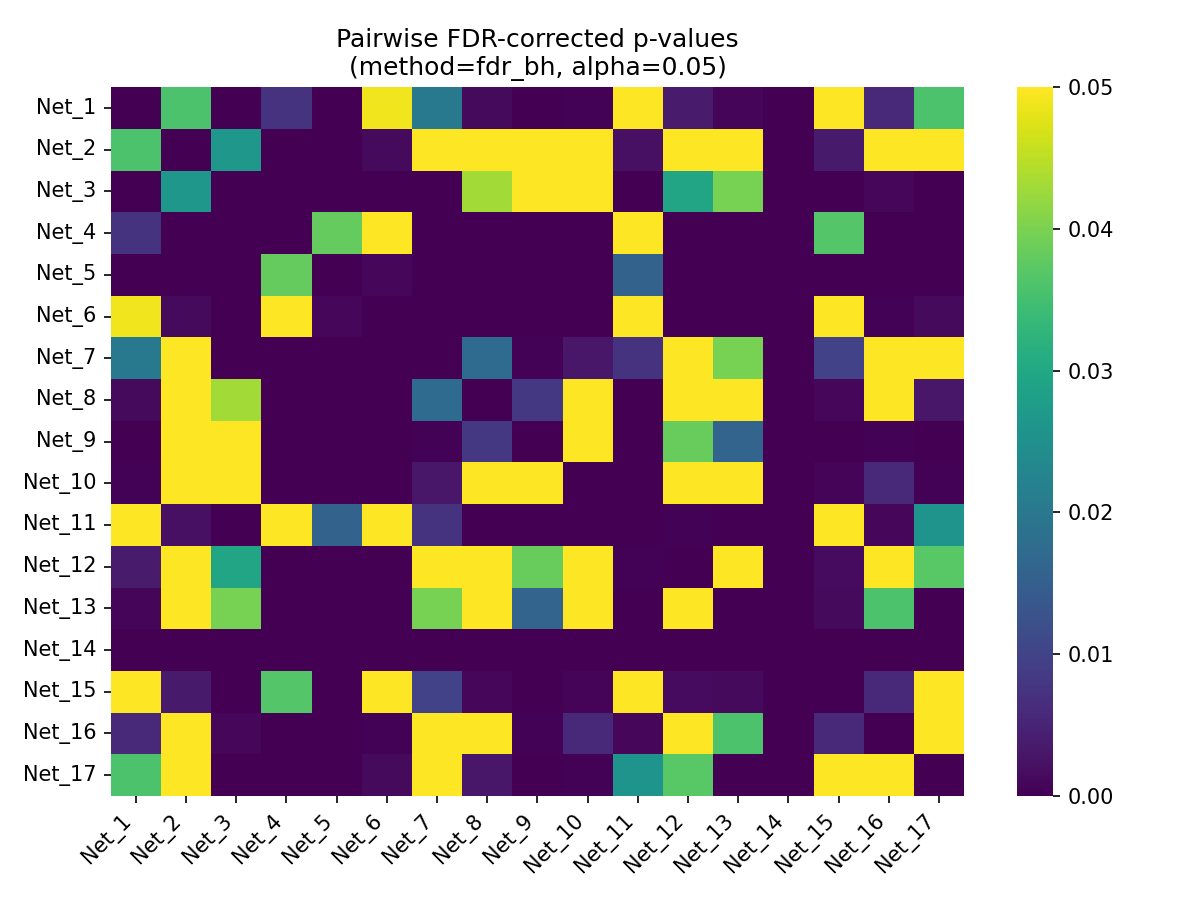
\includegraphics[width=0.65\linewidth]{Results/Plots/Pairwise_Network_Heatmap.png}
\caption{Pairwise FDR-corrected $p$-values ($\alpha=0.05$) among the 17 Yeo networks.}
\label{fig:heatmap}
\end{figure}

Overall, the ISC results indicate that narrative stimuli produce significantly higher neural synchrony across participants, particularly within networks associated with high-level cognitive integration such as the Control/Frontoparietal and Default Mode networks. The large effect sizes and significant ANOVA results underscore the robust impact of narrative content on inter-subject alignment.

\subsection{Cross-Modal RSA}
In this study, data from both EEG and fMRI, and from two conditions (narrative vs. non-narrative), were segmented into fixed-length windows of 10 seconds. For each segment, the average neural pattern was computed and then used to construct a representational dissimilarity matrix (RDM). In this process, the dissimilarity between each pair of segments was calculated as one minus the Pearson correlation coefficient. After the RDMs were constructed for EEG and fMRI separately, I averaged them across subjects to obtain the group-level RDMs for each modality and condition (see Figures \ref{fig:rdm_narr} and  \ref{fig:rdm_non_narr}).

\begin{figure}[ht!]
\centering
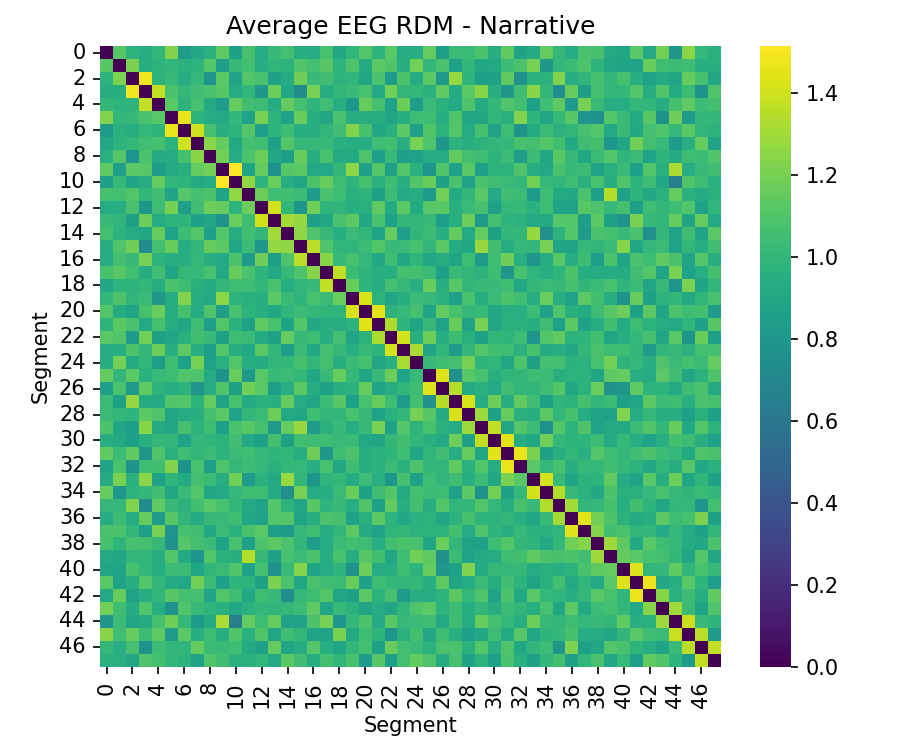
\includegraphics[width=0.45\linewidth]{Results/Plots/Avg_EEG_RDM_narr.png}
\hfill
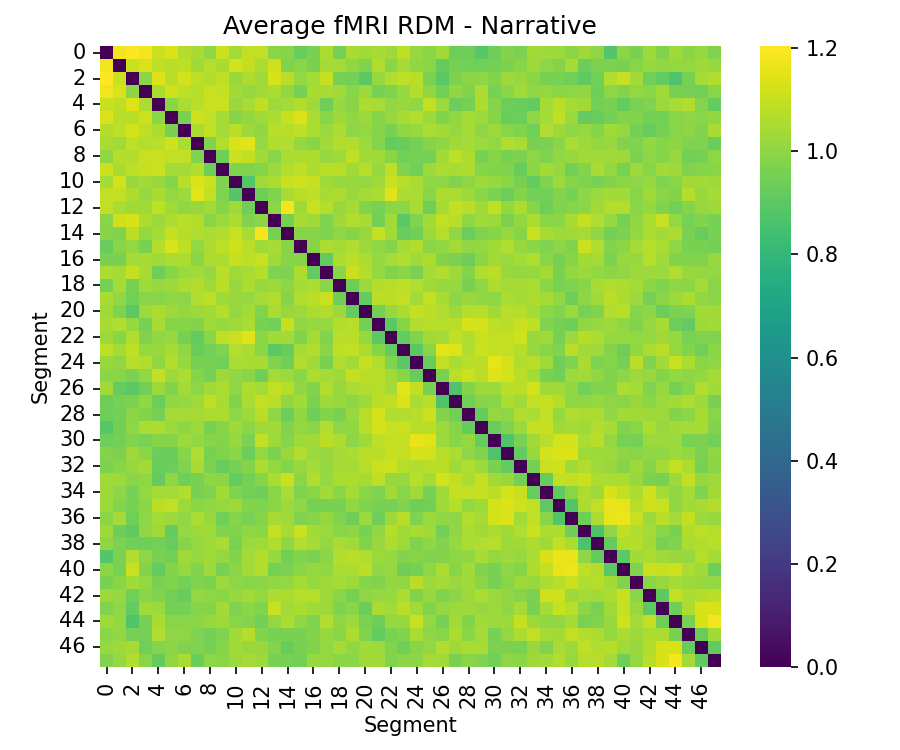
\includegraphics[width=0.45\linewidth]{Results/Plots/Avg_fMRI_RDM_narr.png}
\caption{Average RDMs for the \textbf{narrative} condition. 
\textbf{Left:} EEG RDM (averaged across subjects), 
\textbf{Right:} fMRI RDM (averaged across subjects). 
Each matrix displays the correlation distance (i.e., $1 - \text{Pearson correlation}$) among the 10-second segments along both axes.}
\label{fig:rdm_narr}
\end{figure}

\begin{figure}[ht!]
\centering
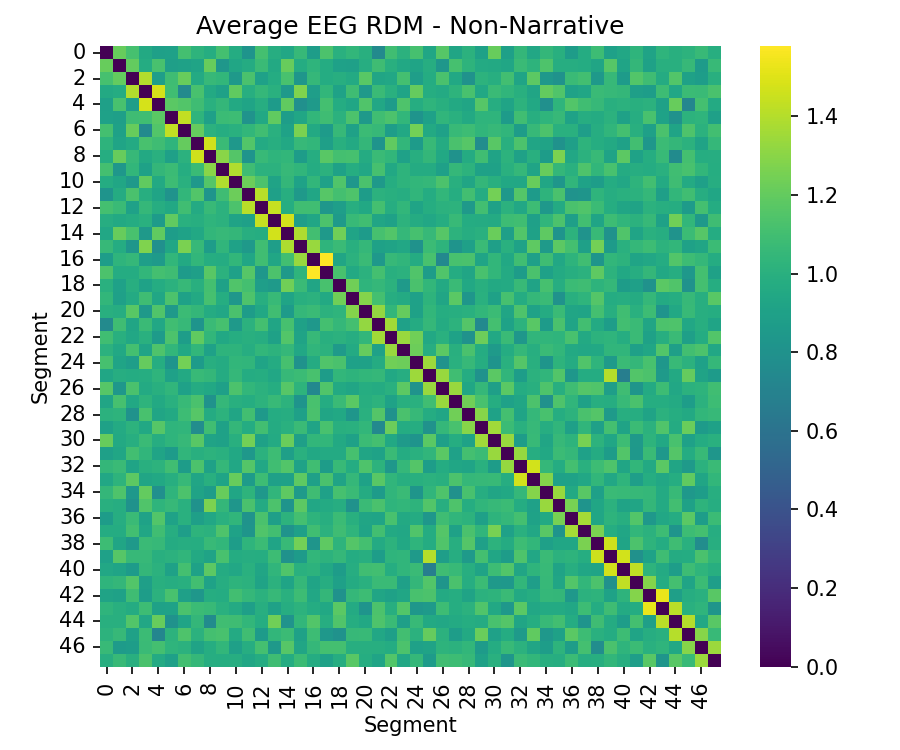
\includegraphics[width=0.45\linewidth]{Results/Plots/Avg_EEG_RDM_non_narr.png}
\hfill
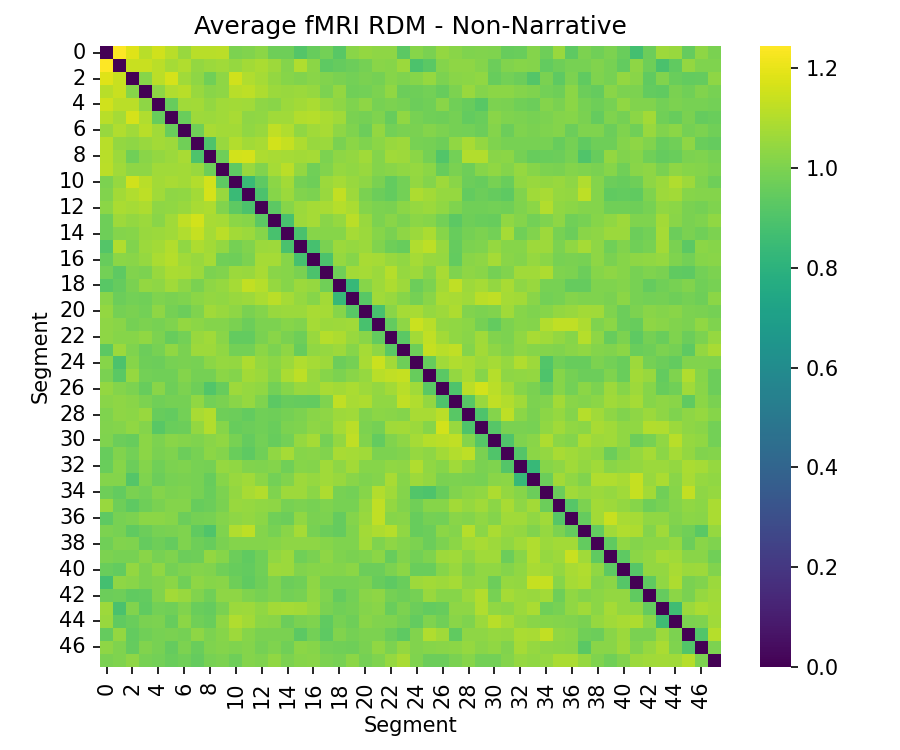
\includegraphics[width=0.45\linewidth]{Results/Plots/Avg_fMRI_RDM_non_narr.png}
\caption{Average RDMs for the \textbf{non-narrative} condition. \textbf{Left:} EEG RDM (averaged across subjects), \textbf{Right:} fMRI RDM (averaged across subjects). Each matrix shows the correlation distance among the 10-second segments for EEG or fMRI.}
\label{fig:rdm_non_narr}
\end{figure}

At the group level, the RSA between the EEG and fMRI data yielded a mean correlation of 0.003 for the narrative condition ($p=0.6736$) and a mean correlation of $-0.009$ for the non-narrative condition ($p=0.02086$). A paired t-test comparing the RSA values between the narrative and non-narrative conditions resulted in $t=1.5057$ with a $p$-value of $0.1478$, indicating that the difference between conditions was not statistically significant. In addition, the classification analysis using the RSA features achieved an accuracy of 52.8\%, which is only marginally above the chance level.

These findings suggest that while the narrative condition exhibits a slight positive trend in cross-modal representational alignment, the overall differences in RSA between narrative and non-narrative conditions remain modest. The modest classification accuracy further implies that the current RSA approach does not provide a robust discriminative signature for narrative versus non-narrative segments under the applied parameters.

\section{Discussion}
Aiming to examine whether coherent narrative stimuli produce stronger neural synchrony than non-narrative stimuli, as well as to evaluate whether cross-modal representational similarity between EEG and fMRI data differs between these conditions, this study received mixed results answering these two questions. On the one hand, the ISC analysis provided robust evidence supporting the first research question. Specifically, 16 out of the 17 Yeo networks exhibited significantly higher ISC for narrative stimuli, with particularly large effects observed in high-order networks such as the Control/Frontoparietal (Network 14) and Default Mode networks. These findings reinforce previous literature suggesting that narrative content, with its inherent coherence of plot and emotional structure, powerfully aligns neural activity across individuals, especially in networks involved in cognitive integration and semantic processing.

On the other hand, however, the cross-modal RSA analysis yielded only modest differences between narrative and non-narrative conditions. Although the narrative condition showed a slight positive trend (mean RSA of 0.003) compared to a negative trend for non-narrative stimuli (mean RSA of $-0.009$), the paired t-test did not reveal a statistically significant difference ($p=0.1478$). Furthermore, the classification accuracy based on RSA features was near chance (52.8\%). These results suggest that, under the current analysis parameters, the representational alignment between EEG and fMRI does not robustly distinguish between narrative and non-narrative segments. This discrepancy may be due to differences in temporal resolution between EEG and fMRI, the choice of segmentation window, or the insufficient alignment of neural signals across modalities.

Despite the strong ISC findings, several limitations must be considered. First, the current RSA approach may require further refinement; future studies could benefit from optimizing the segmentation strategy, incorporating time-lag adjustments, or focusing on frequency-specific EEG features to better capture the temporal dynamics associated with narrative processing. Second, the modest classification accuracy indicates that additional features or multimodal fusion techniques could be needed to enhance the discriminative power of RSA measures. Lastly, the sample size and variability in the scan intervals between subjects can contribute to noise in the RSA metrics. Future work should explore larger, more homogeneous datasets and incorporate advanced computational methods to further unravel the complex relationship between narrative content and cross-modal neural representations.

\printbibliography

\end{document}